% Requires \usepackage{subcaption} in the preamble (and graphicx).
% Assumes the 8 geo_top20_<model>_shared_scale.png files and
% shared_colorbar.png sit alongside this .tex file (adjust the graphics
% path / \graphicspath as needed for your document tree).
\begin{figure}[htbp]
\centering
  \begin{subfigure}[t]{0.23\textwidth}
    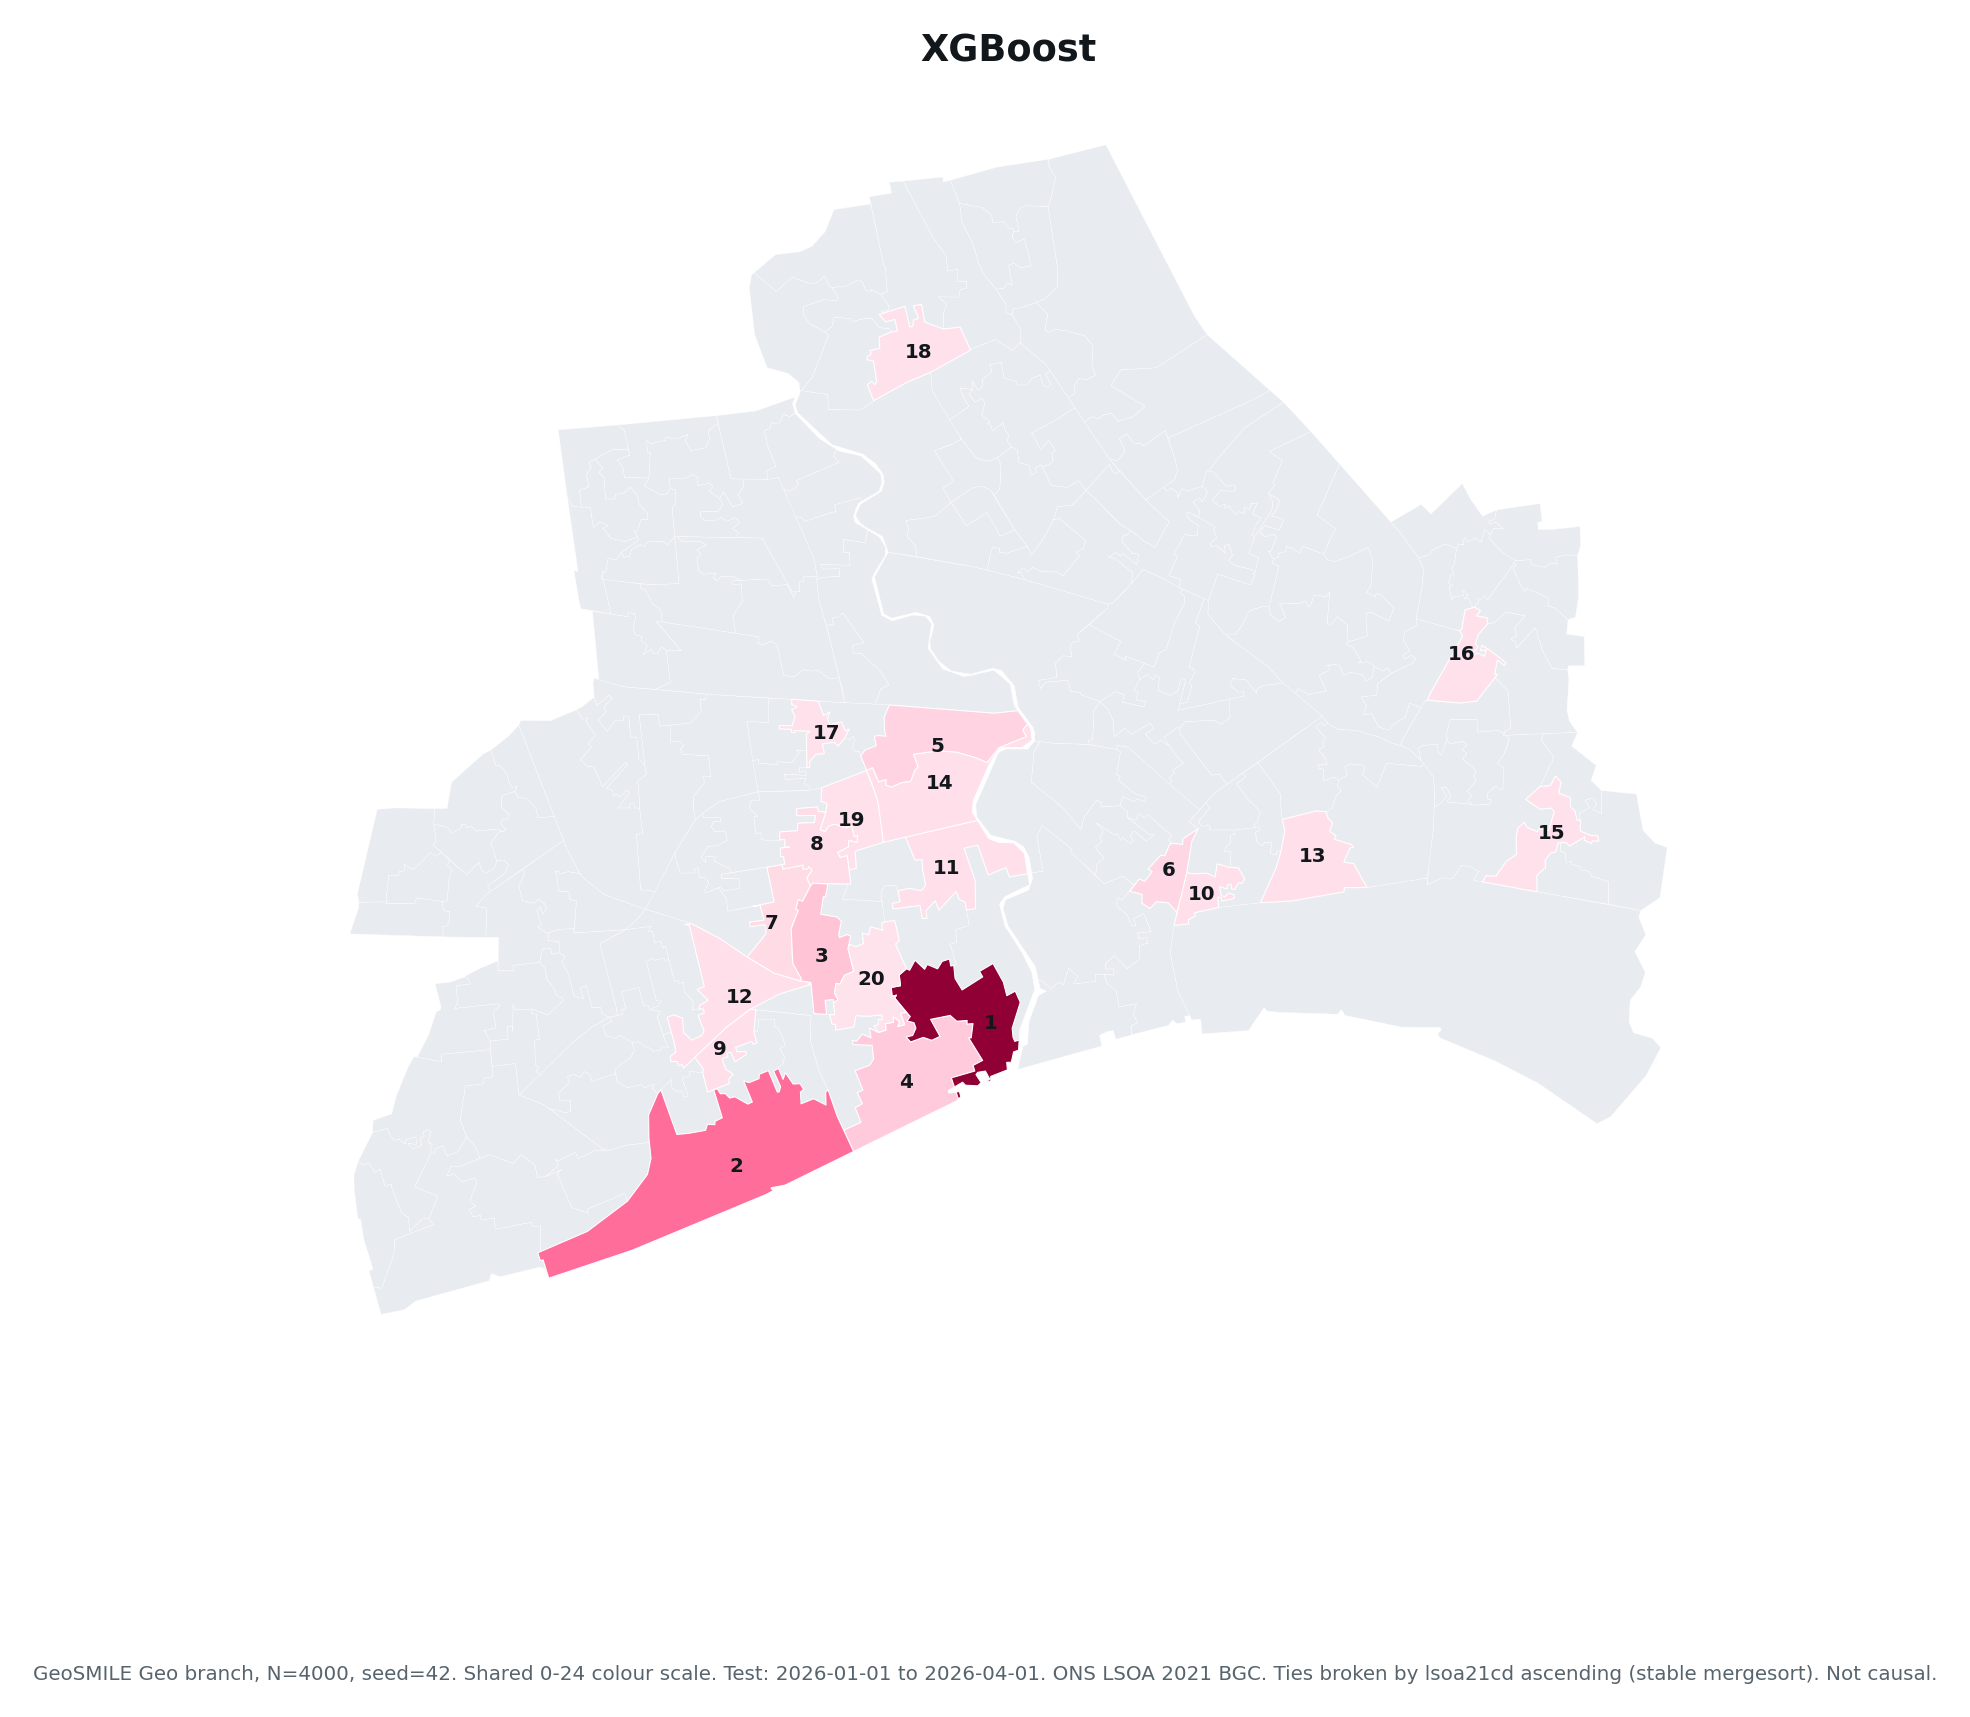
\includegraphics[width=\textwidth]{geo_top20_xgboost_shared_scale.png}
    \subcaption{XGBoost$^{\dagger}$}
    \label{fig:sel_maps_xgboost}
  \end{subfigure} \hfill
  \begin{subfigure}[t]{0.23\textwidth}
    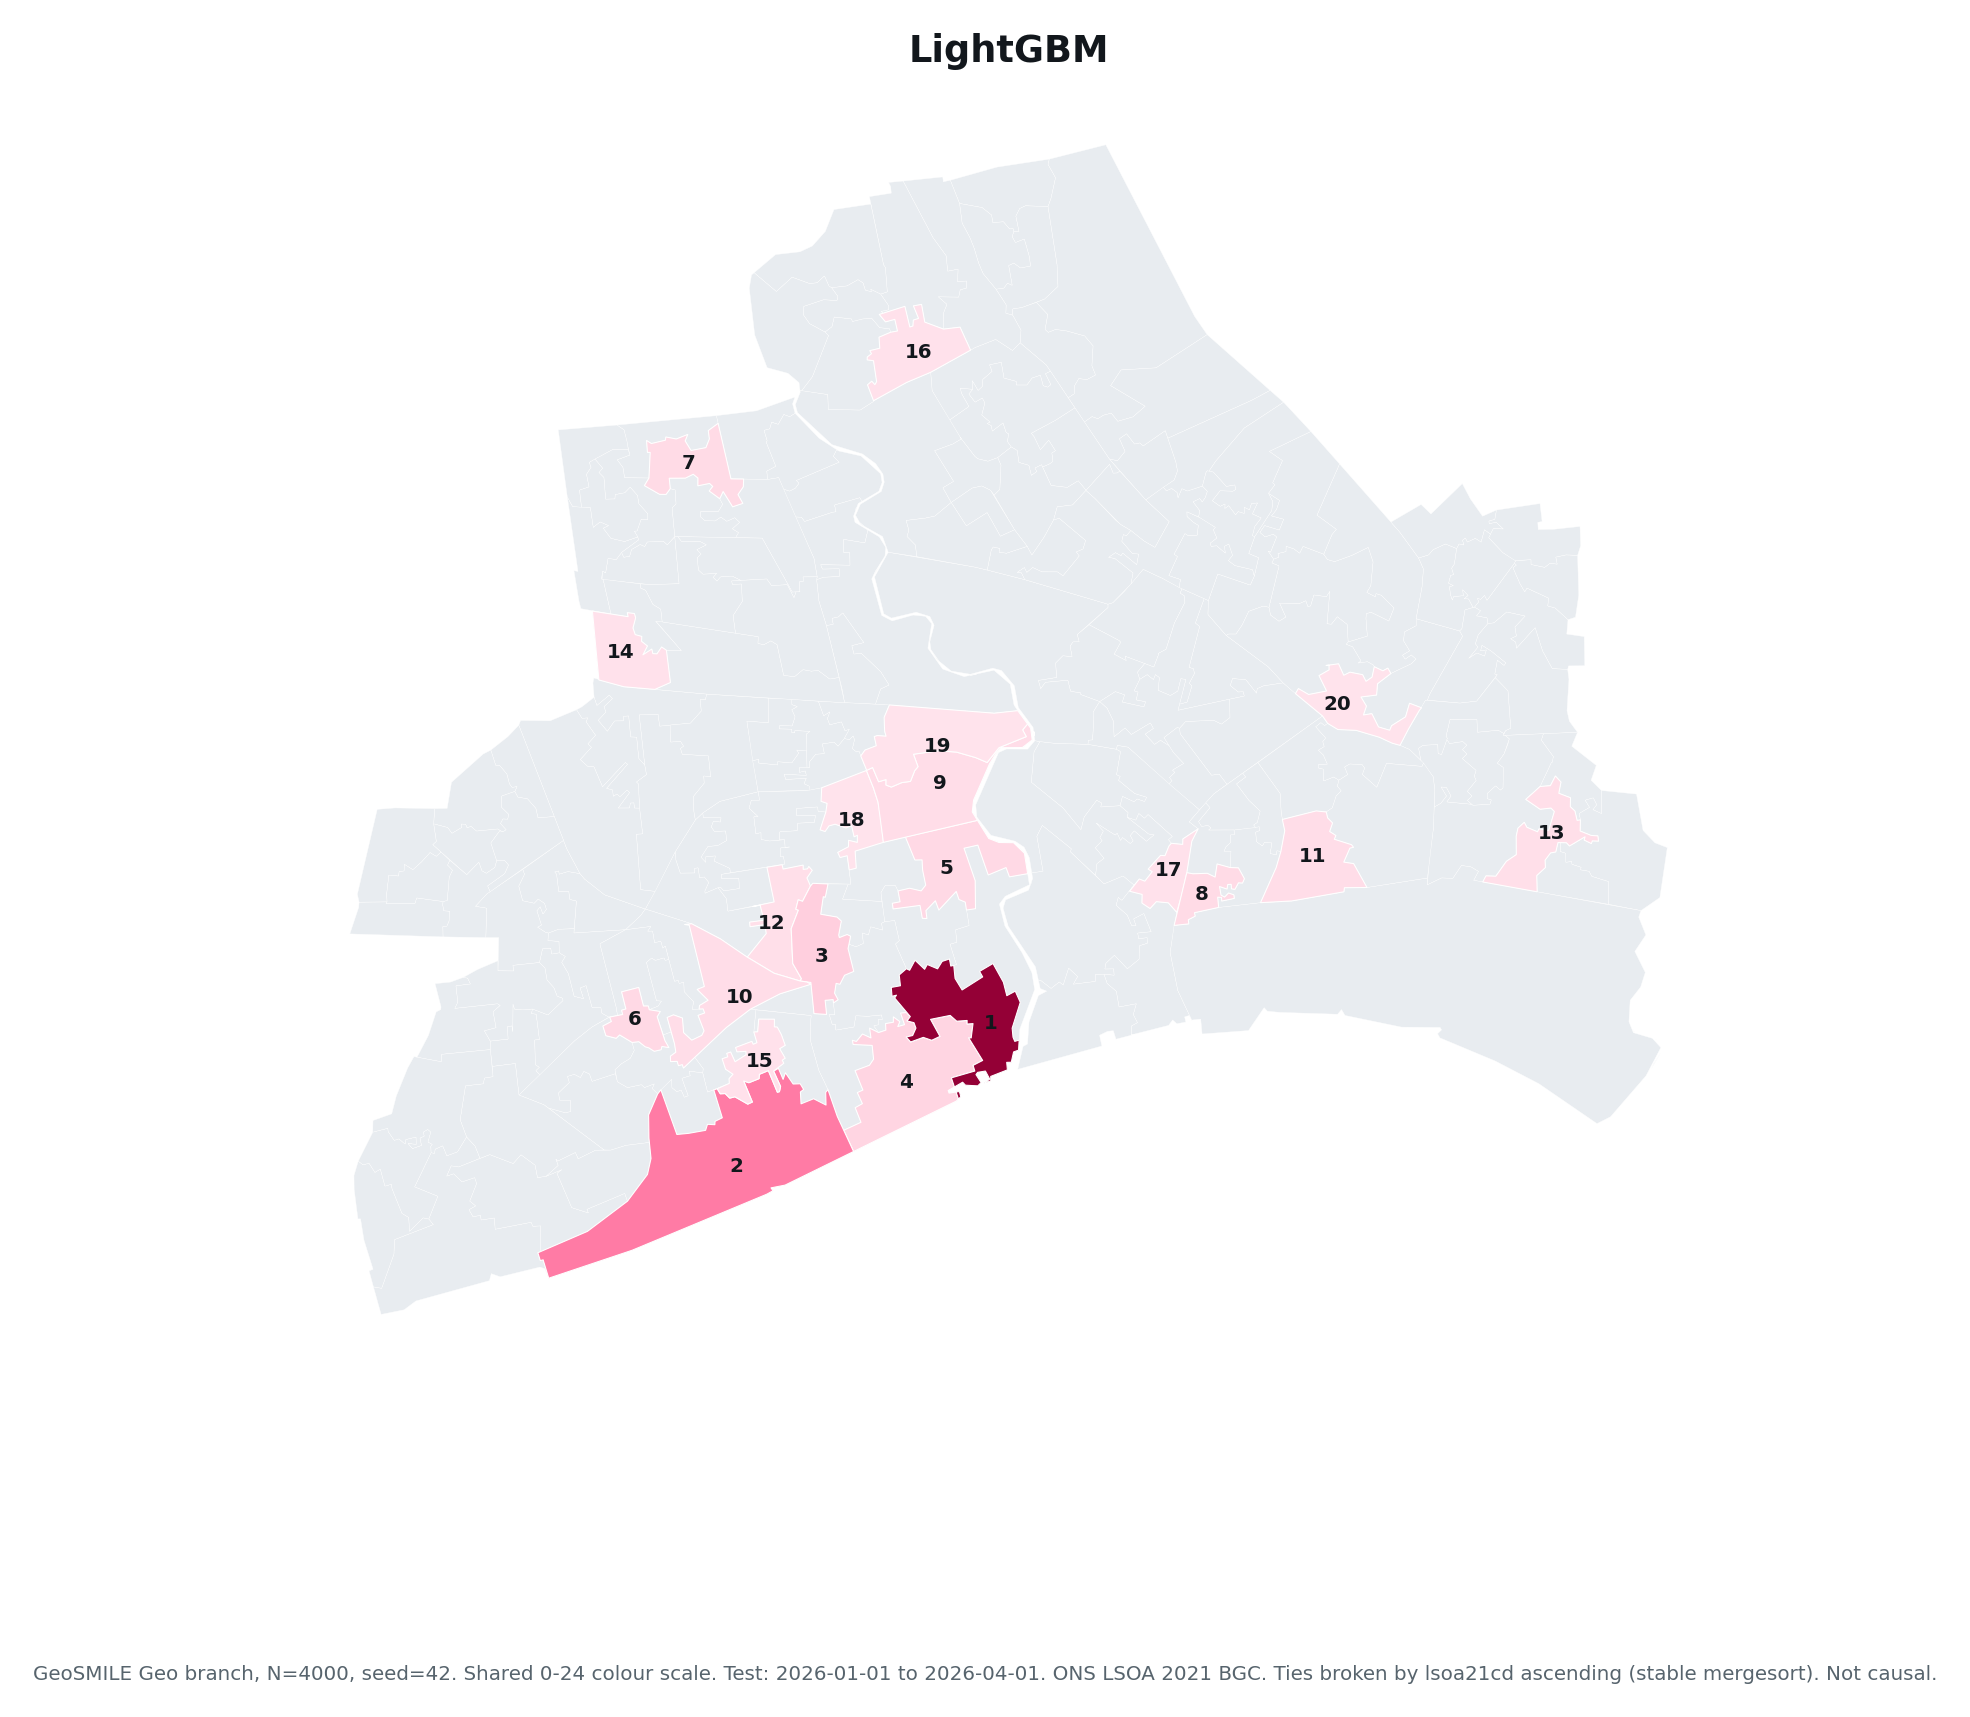
\includegraphics[width=\textwidth]{geo_top20_lightgbm_shared_scale.png}
    \subcaption{LightGBM$^{\dagger}$}
    \label{fig:sel_maps_lightgbm}
  \end{subfigure} \hfill
  \begin{subfigure}[t]{0.23\textwidth}
    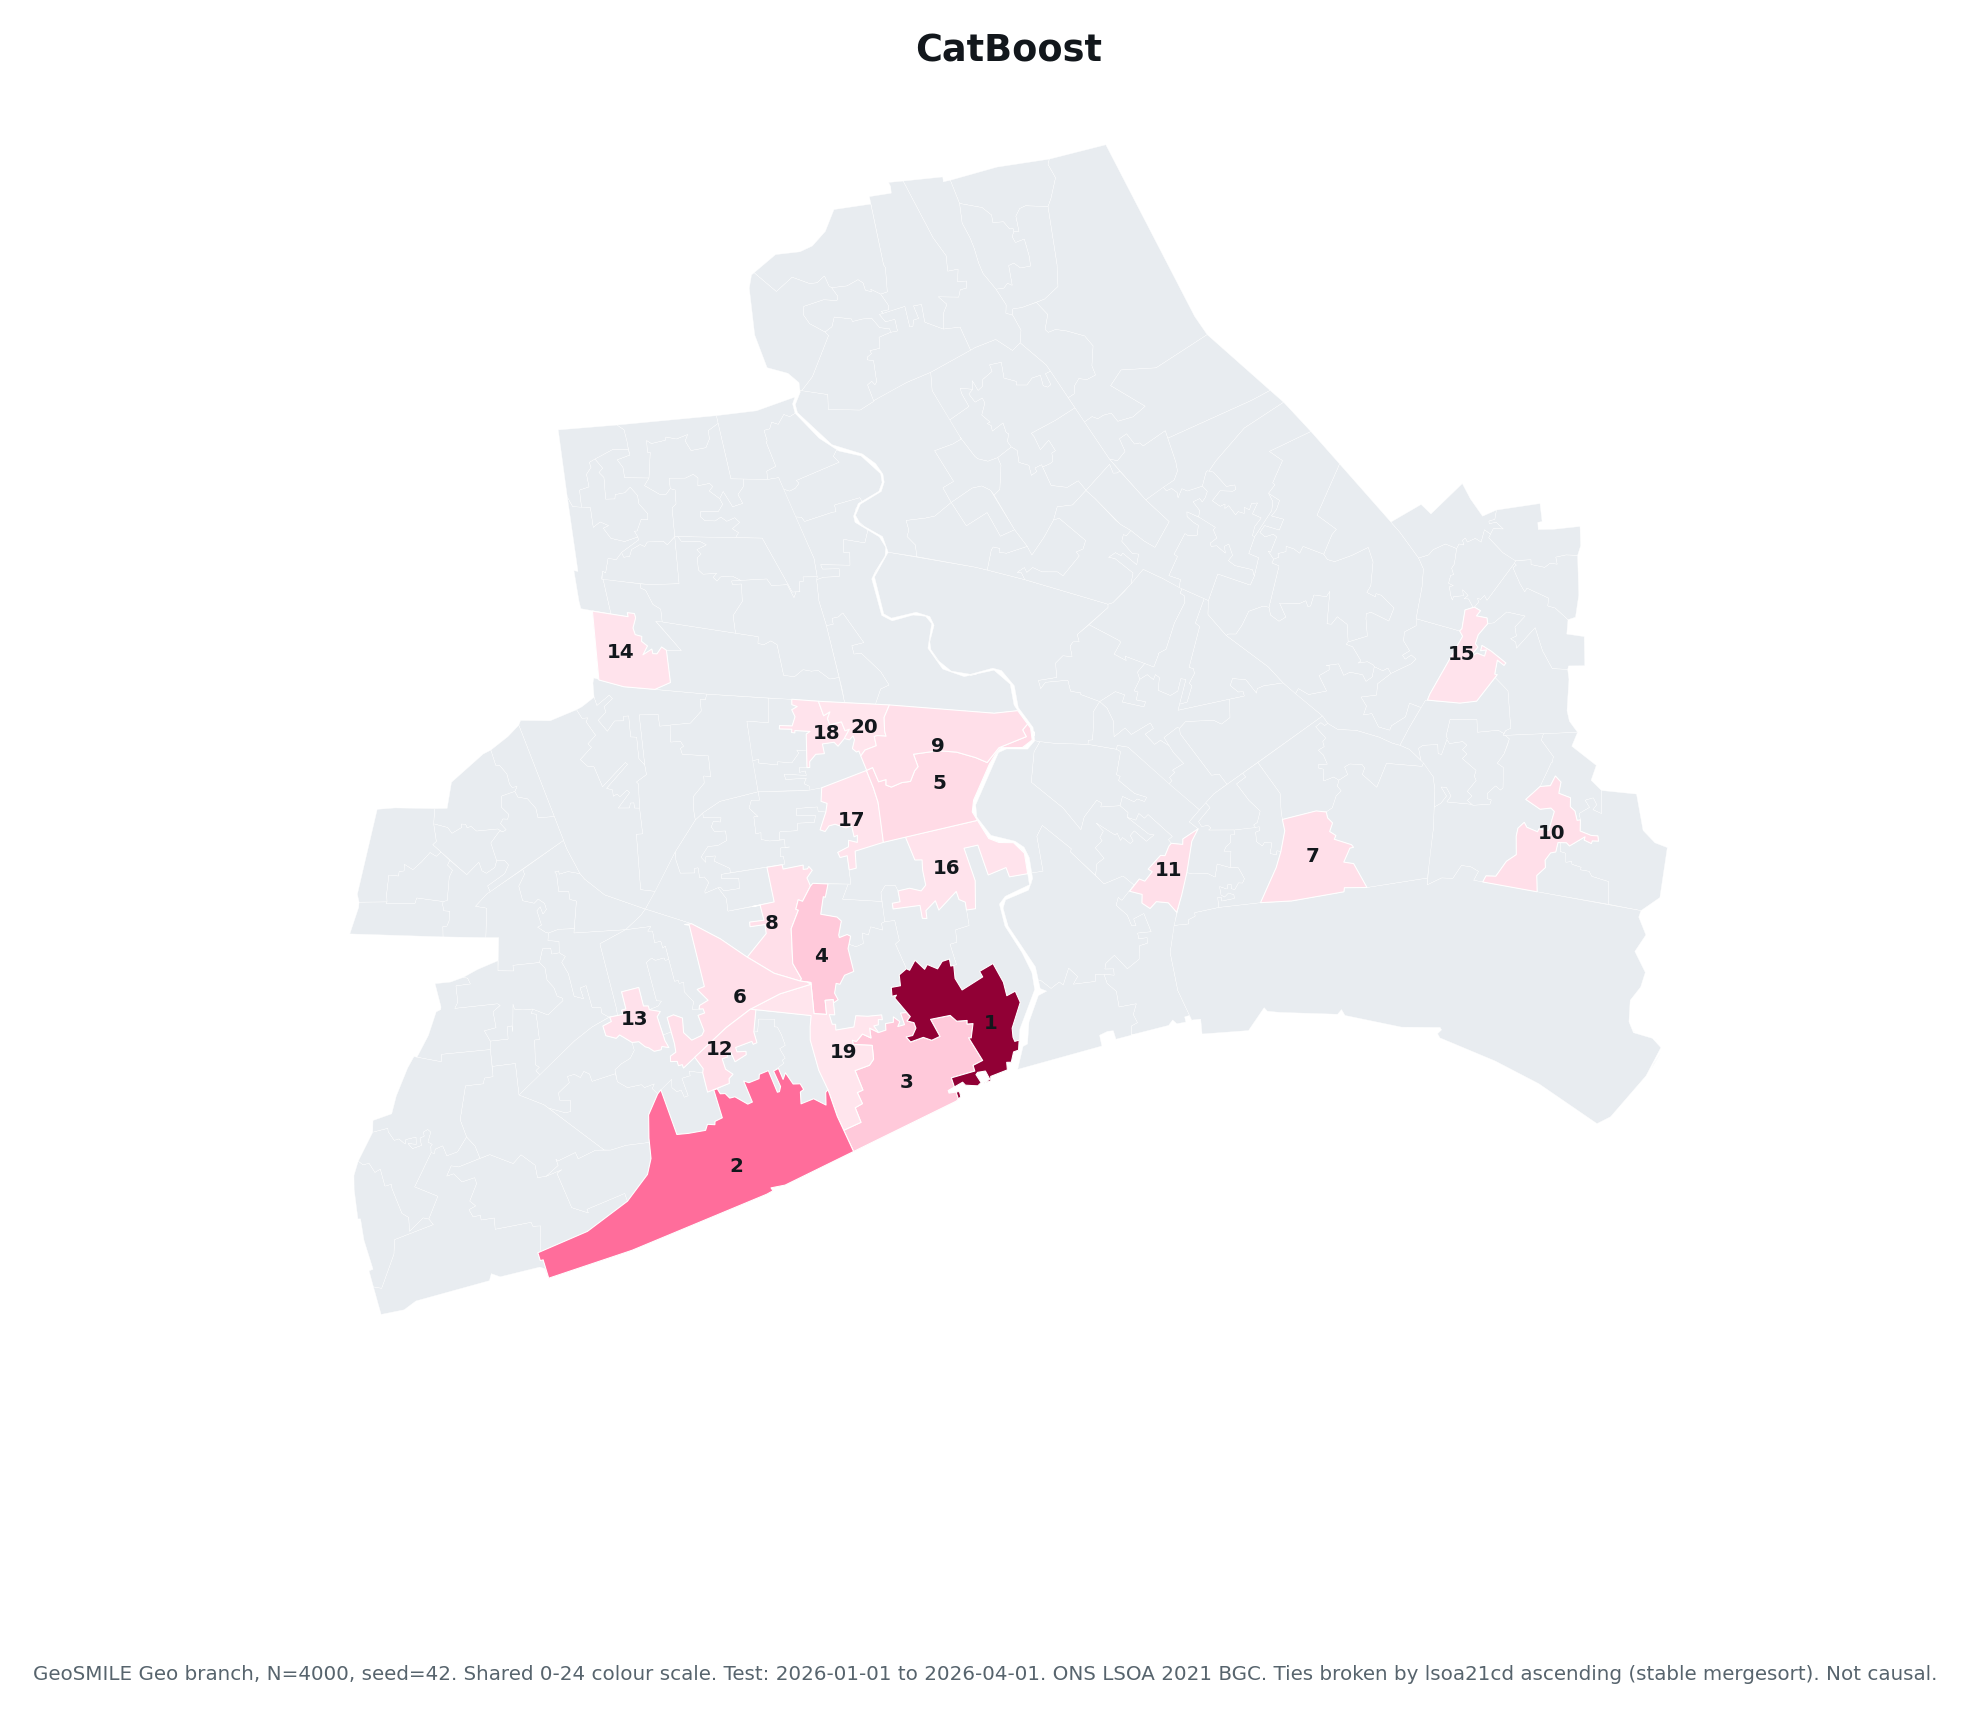
\includegraphics[width=\textwidth]{geo_top20_catboost_shared_scale.png}
    \subcaption{CatBoost$^{\dagger}$}
    \label{fig:sel_maps_catboost}
  \end{subfigure} \hfill
  \begin{subfigure}[t]{0.23\textwidth}
    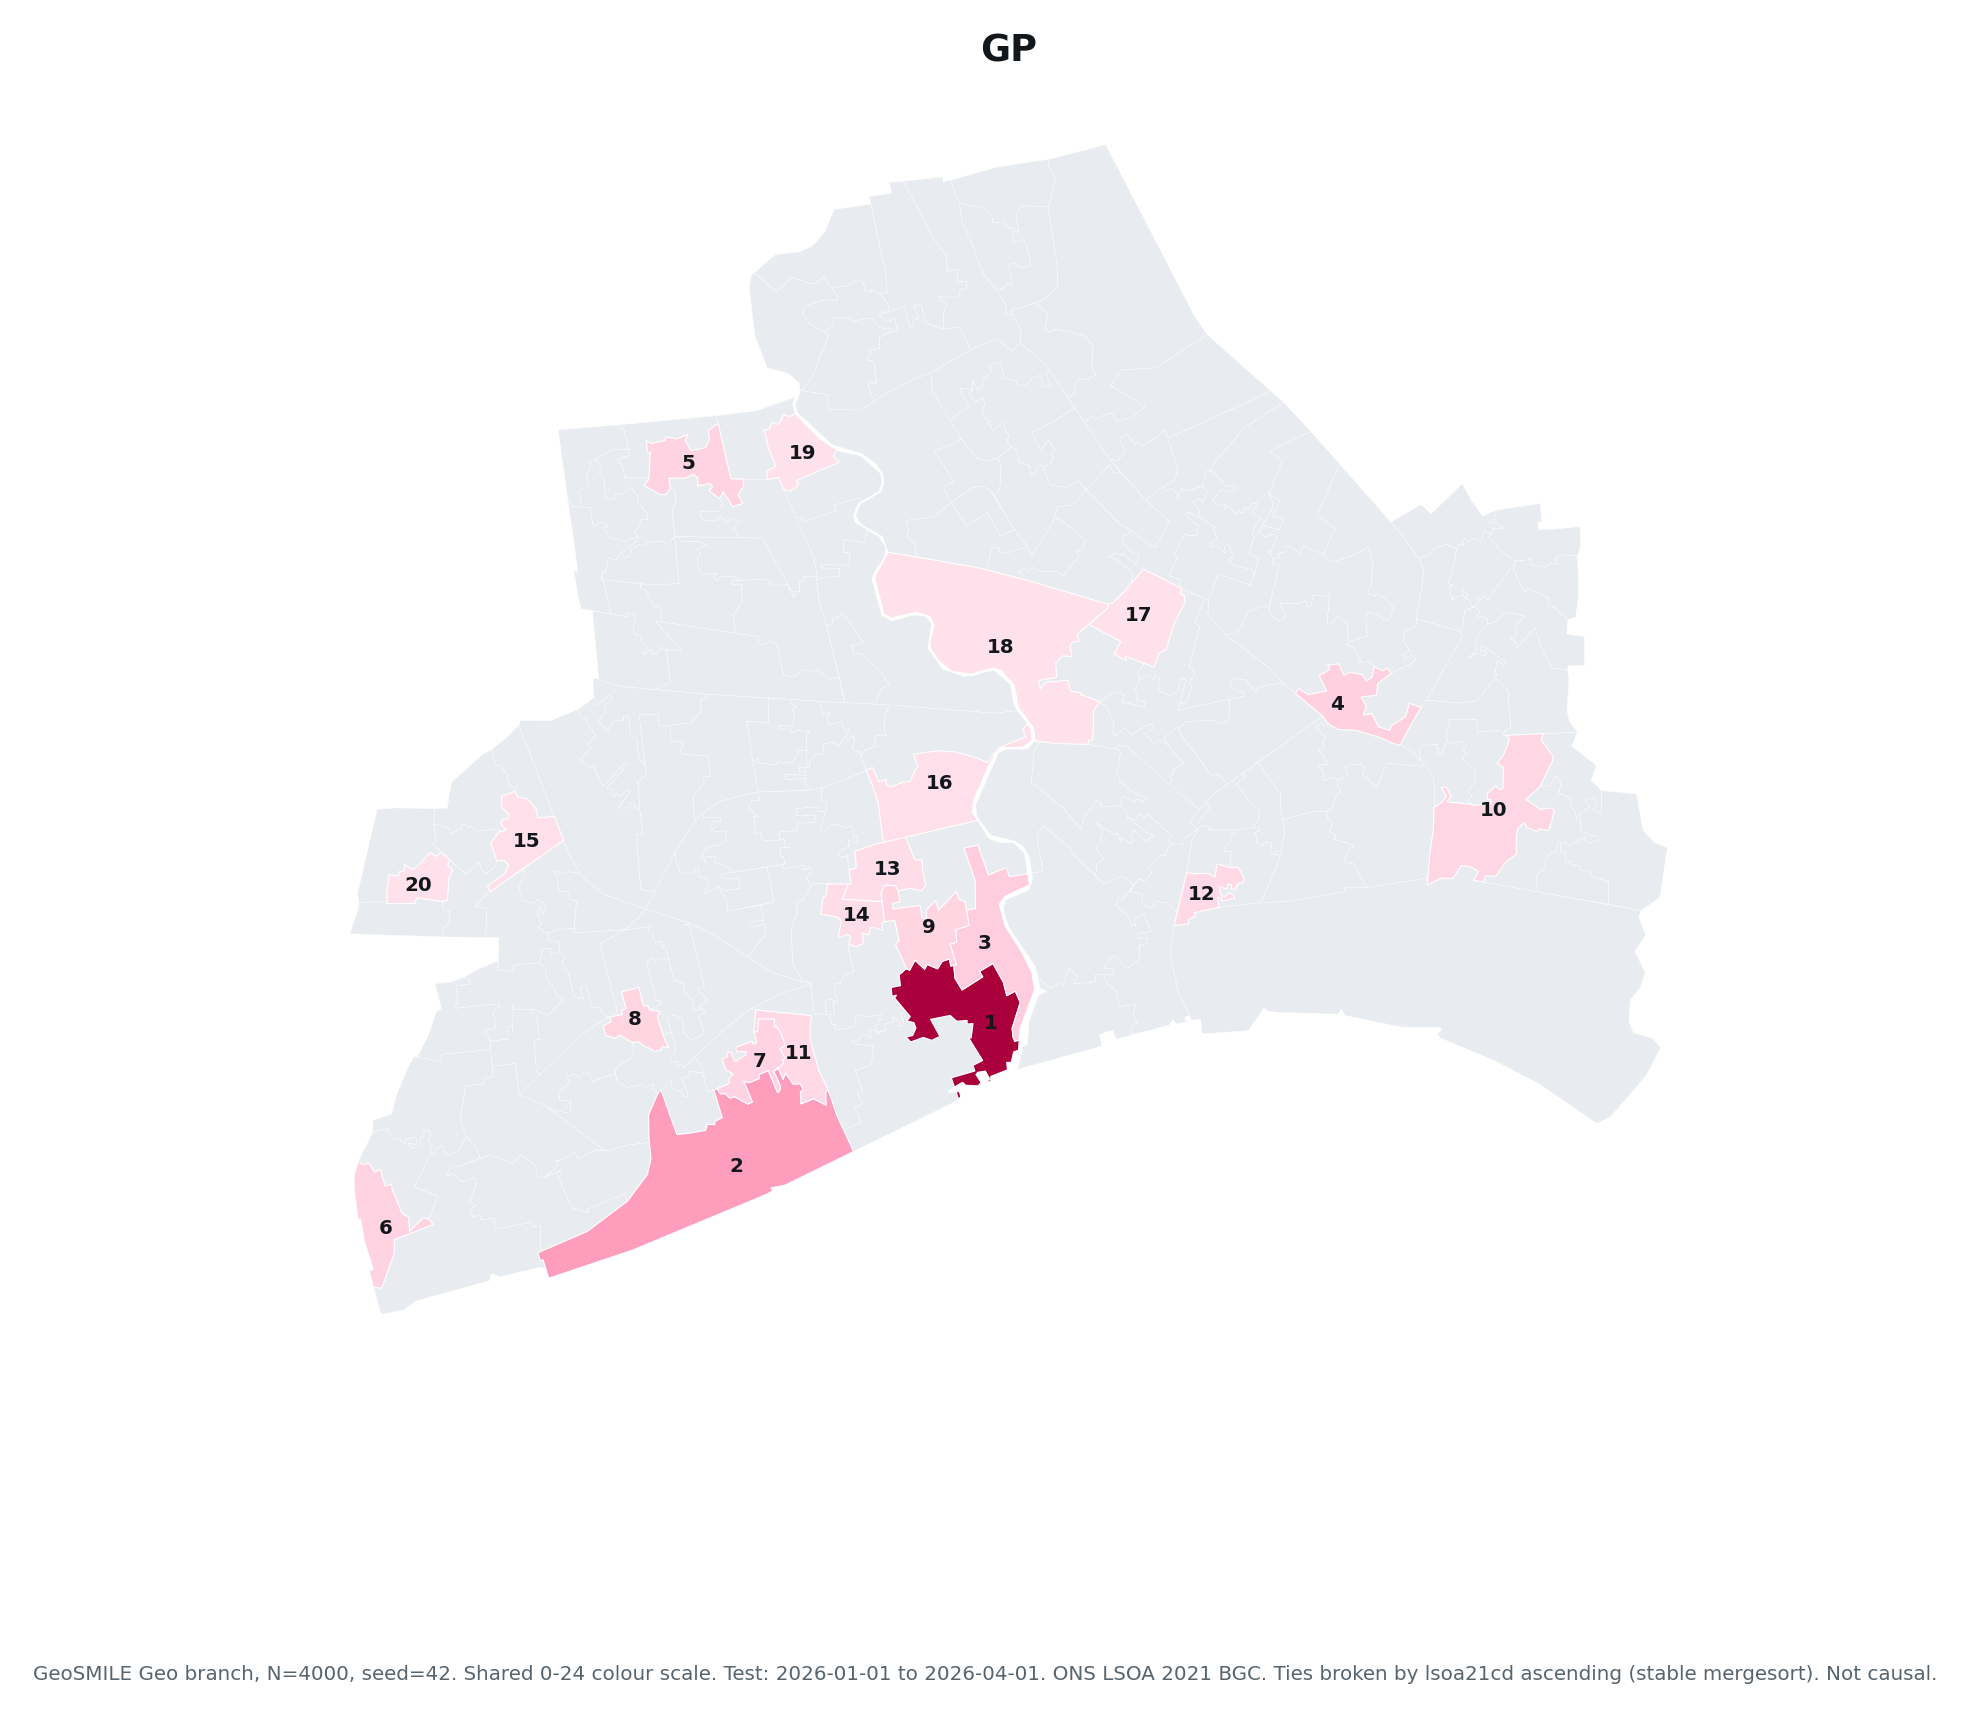
\includegraphics[width=\textwidth]{geo_top20_gp_shared_scale.png}
    \subcaption{GP$^{\dagger}$}
    \label{fig:sel_maps_gp}
  \end{subfigure}

  \vspace{0.6em}

  \begin{subfigure}[t]{0.23\textwidth}
    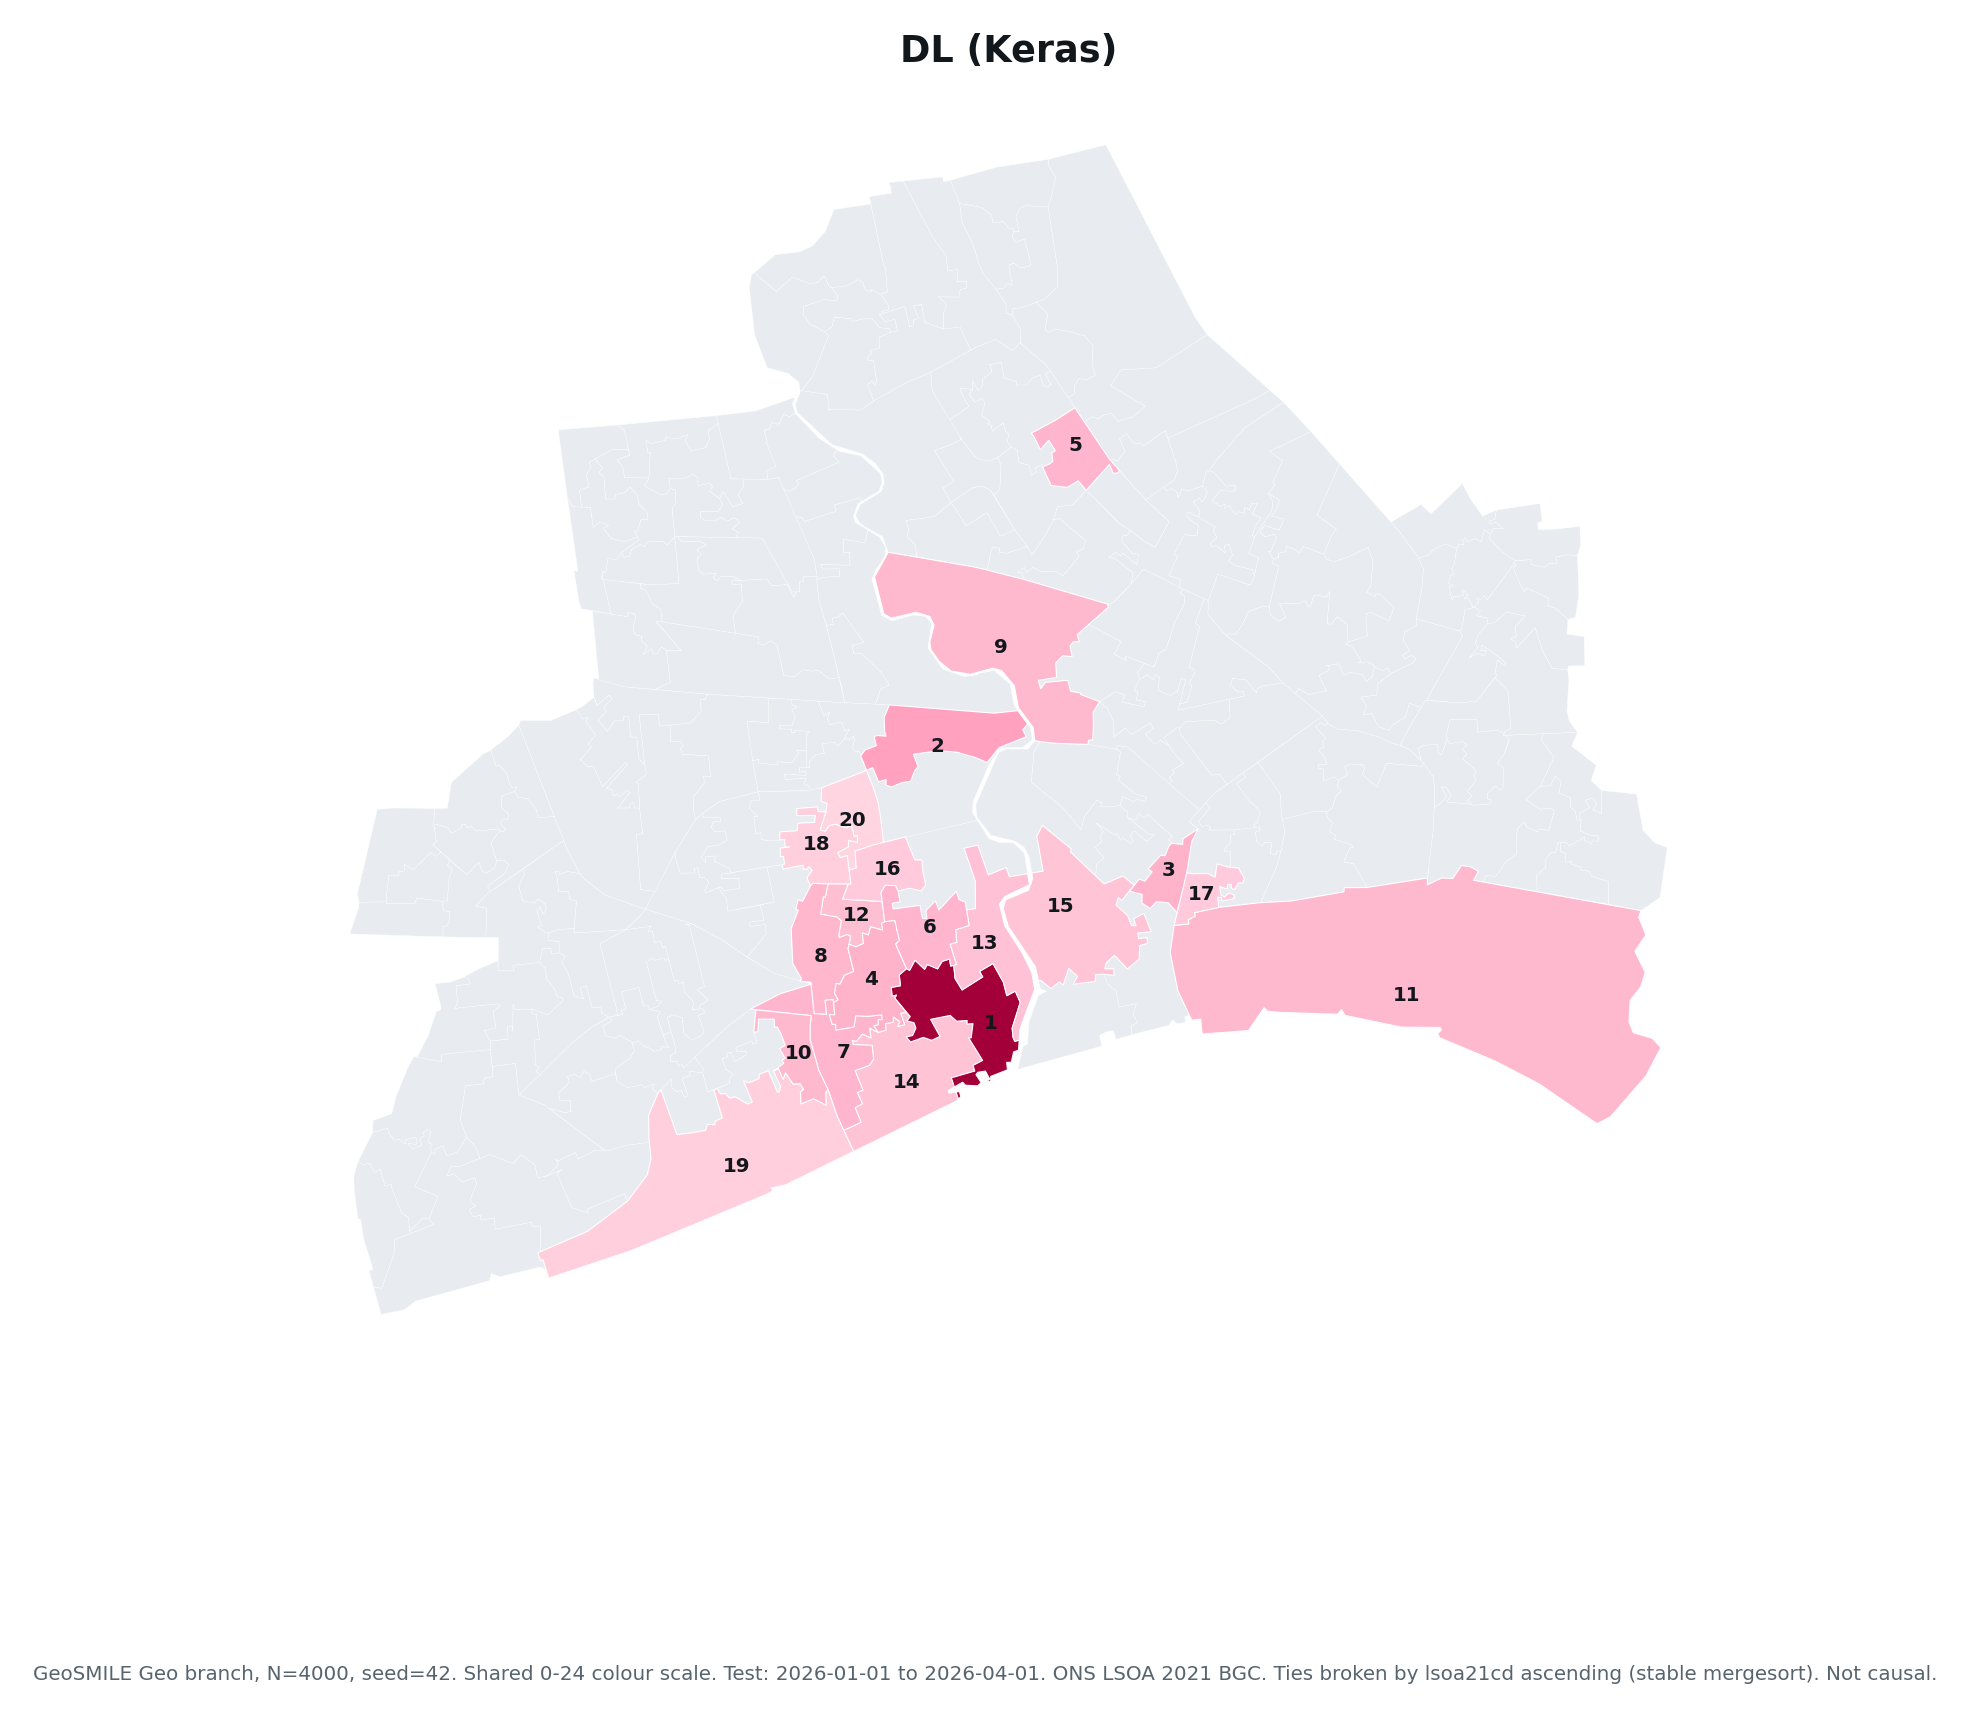
\includegraphics[width=\textwidth]{geo_top20_dl_shared_scale.png}
    \subcaption{DL (Keras)$^{\dagger}$}
    \label{fig:sel_maps_dl}
  \end{subfigure} \hfill
  \begin{subfigure}[t]{0.23\textwidth}
    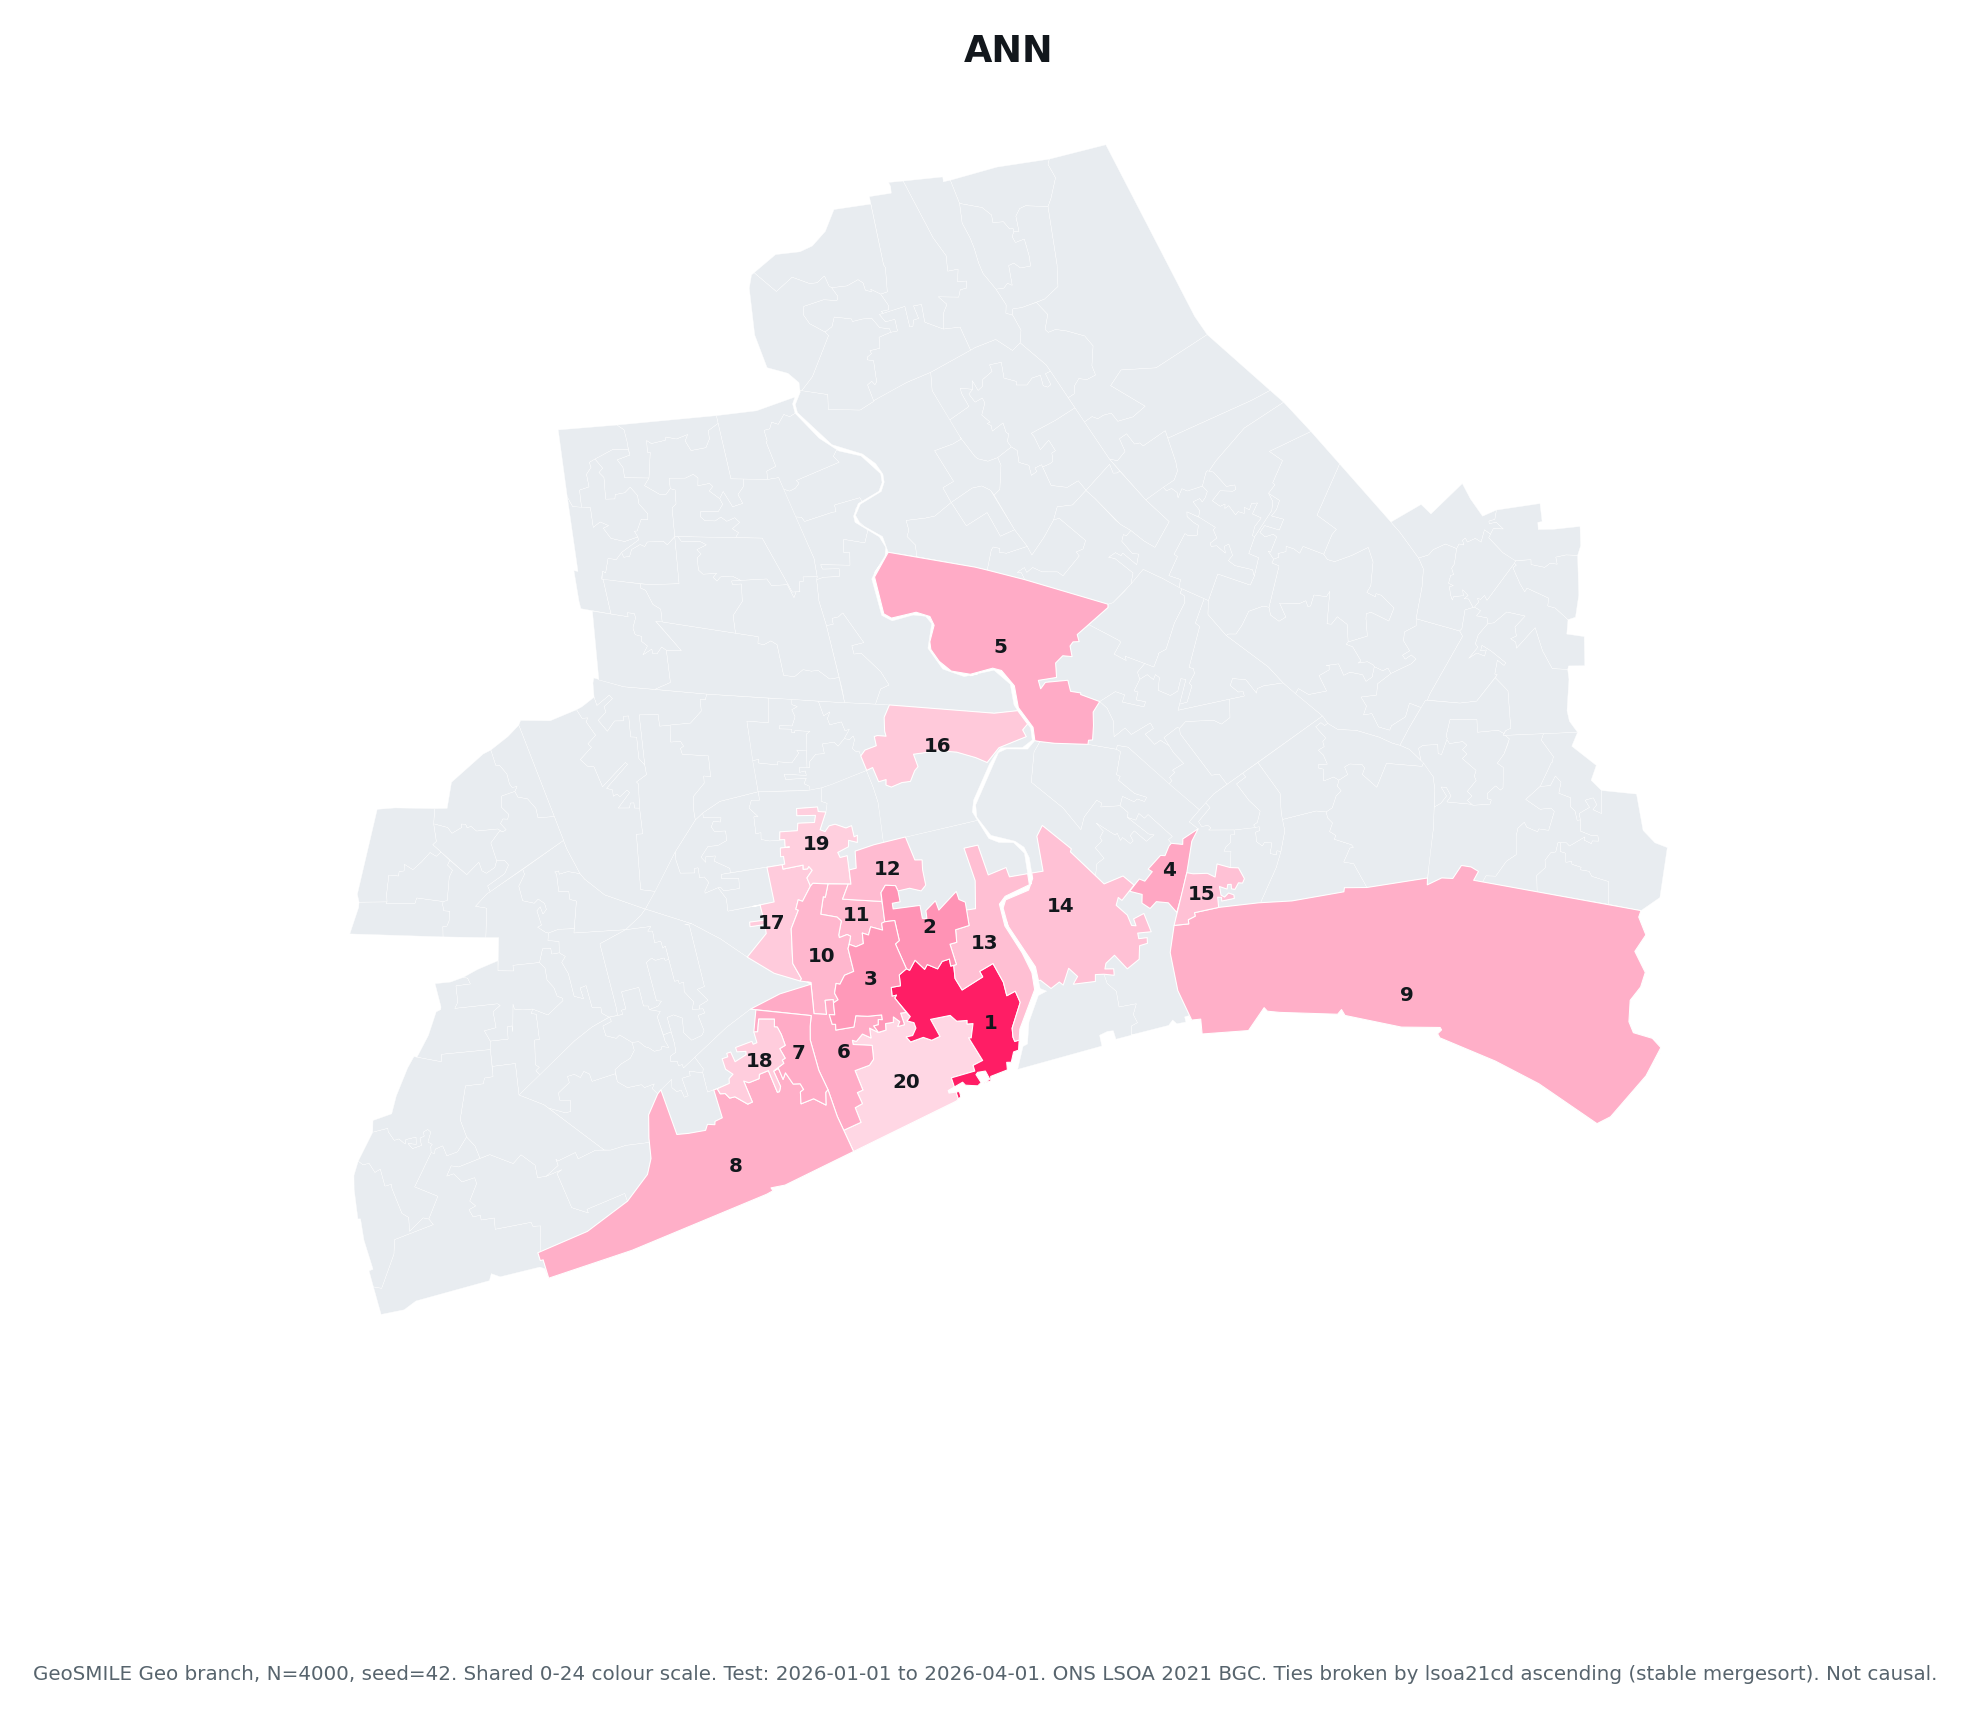
\includegraphics[width=\textwidth]{geo_top20_ann_shared_scale.png}
    \subcaption{ANN$^{\ddagger}$}
    \label{fig:sel_maps_ann}
  \end{subfigure} \hfill
  \begin{subfigure}[t]{0.23\textwidth}
    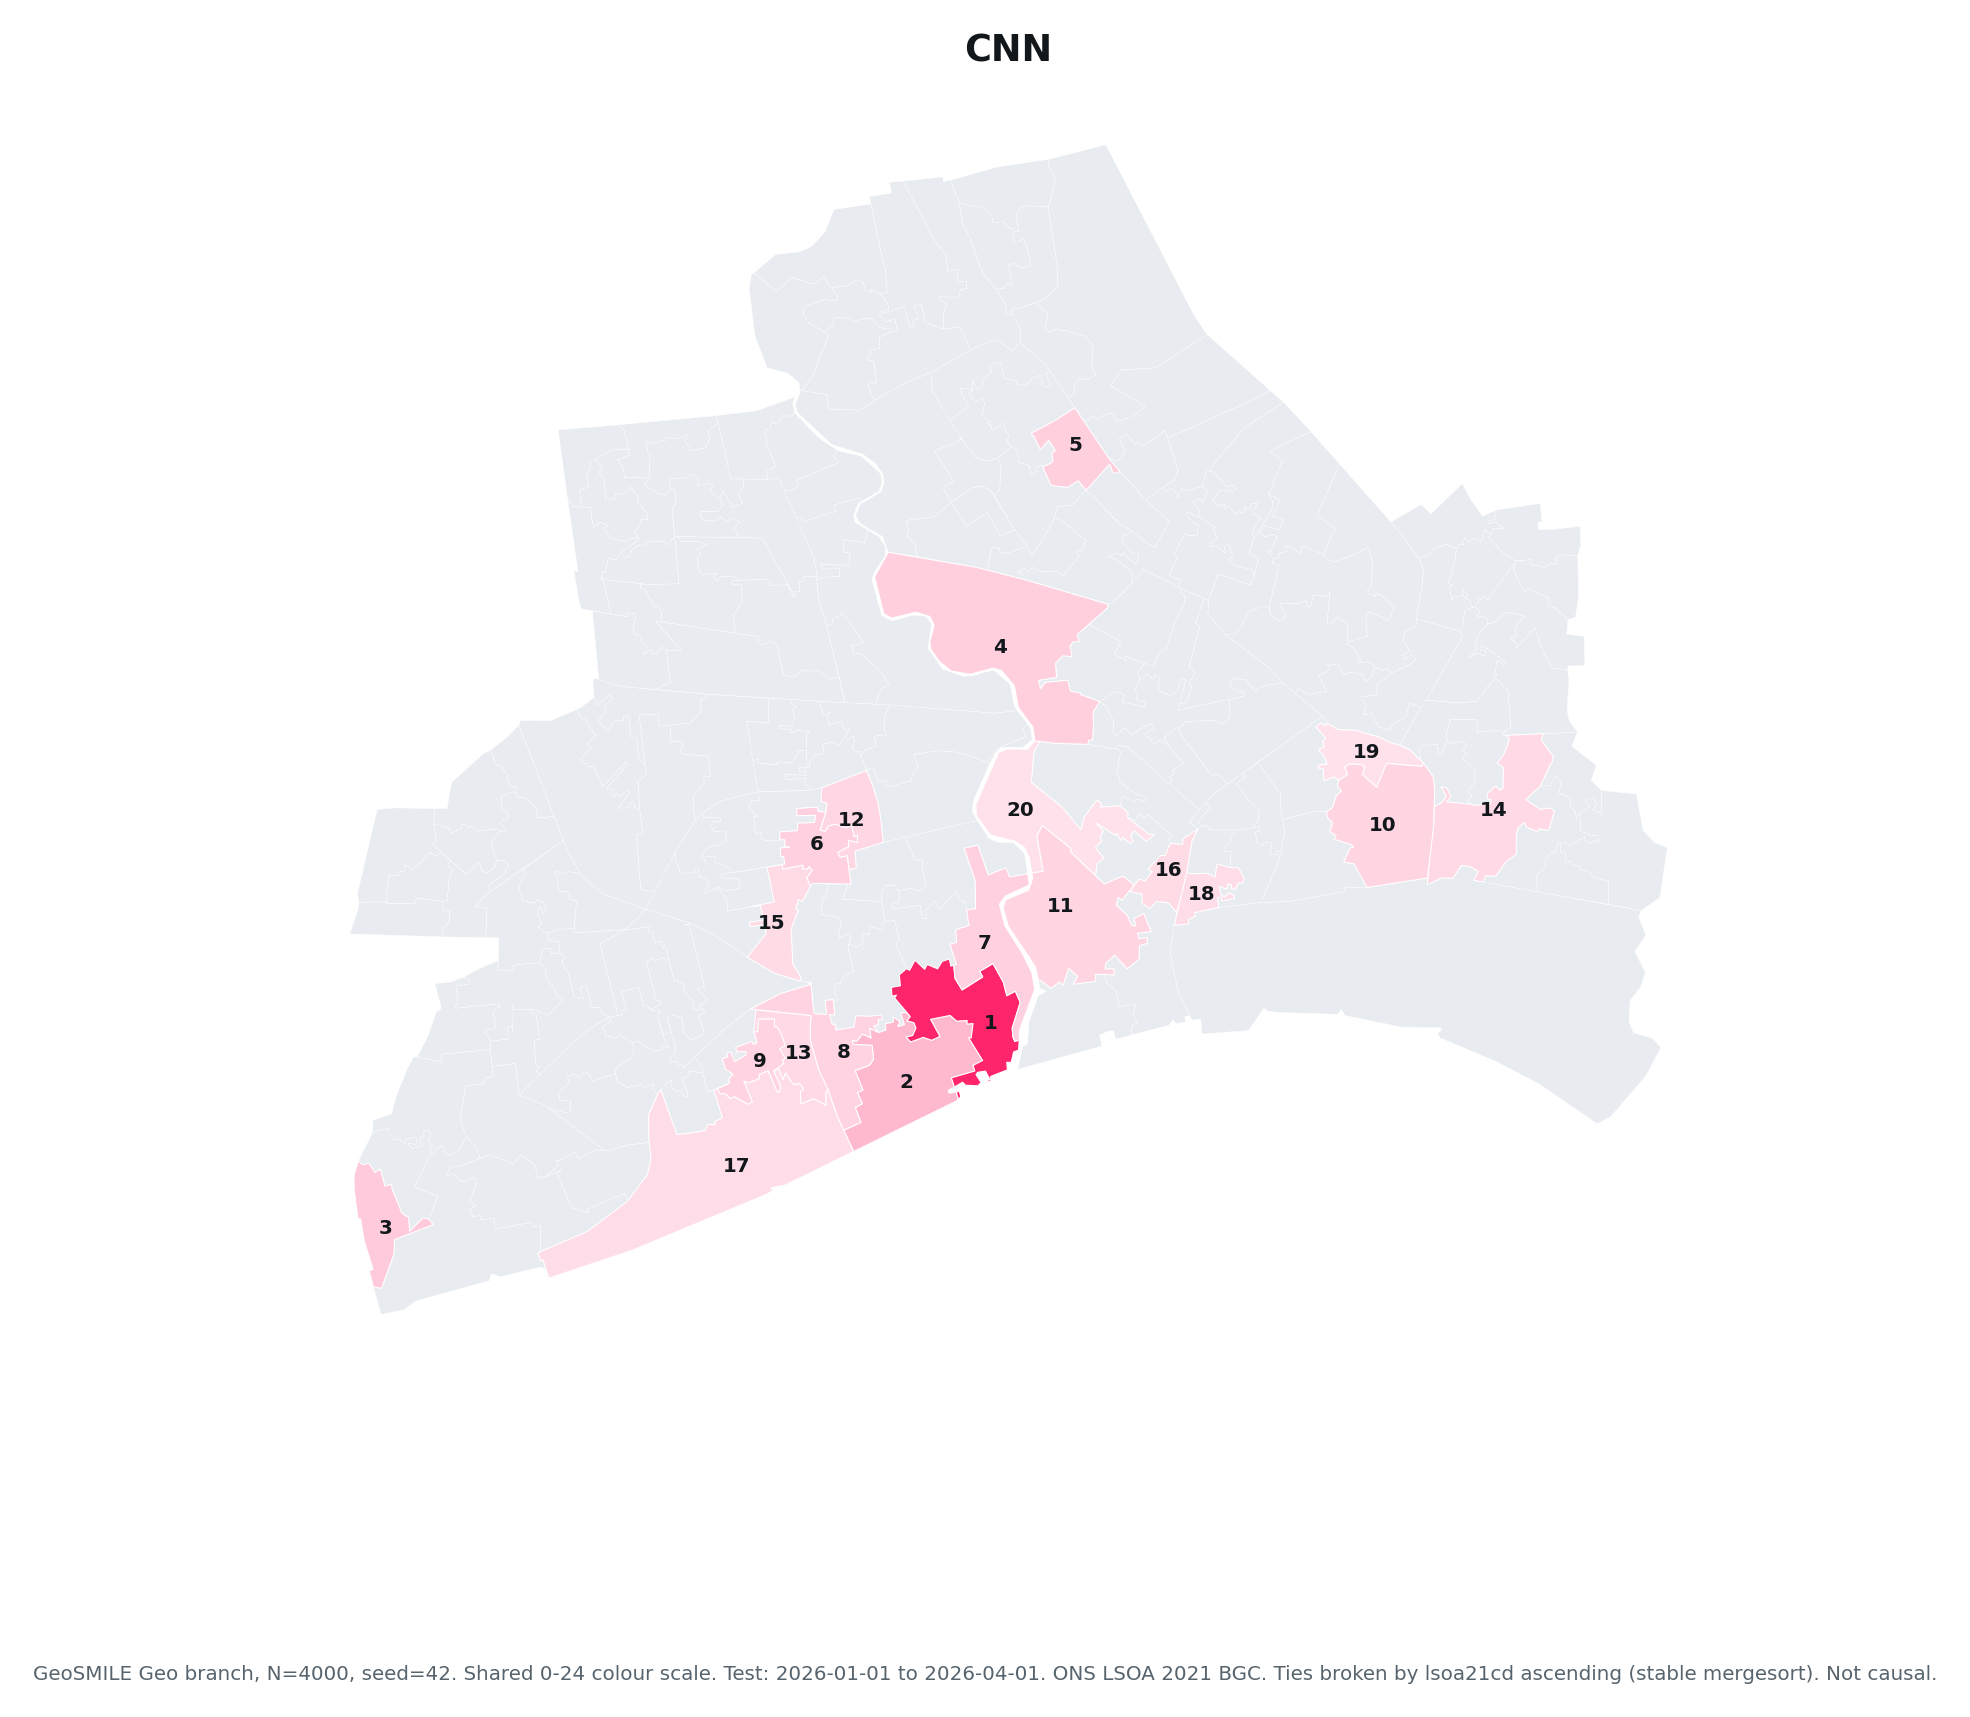
\includegraphics[width=\textwidth]{geo_top20_cnn_shared_scale.png}
    \subcaption{CNN$^{\S}$}
    \label{fig:sel_maps_cnn}
  \end{subfigure} \hfill
  \begin{subfigure}[t]{0.23\textwidth}
    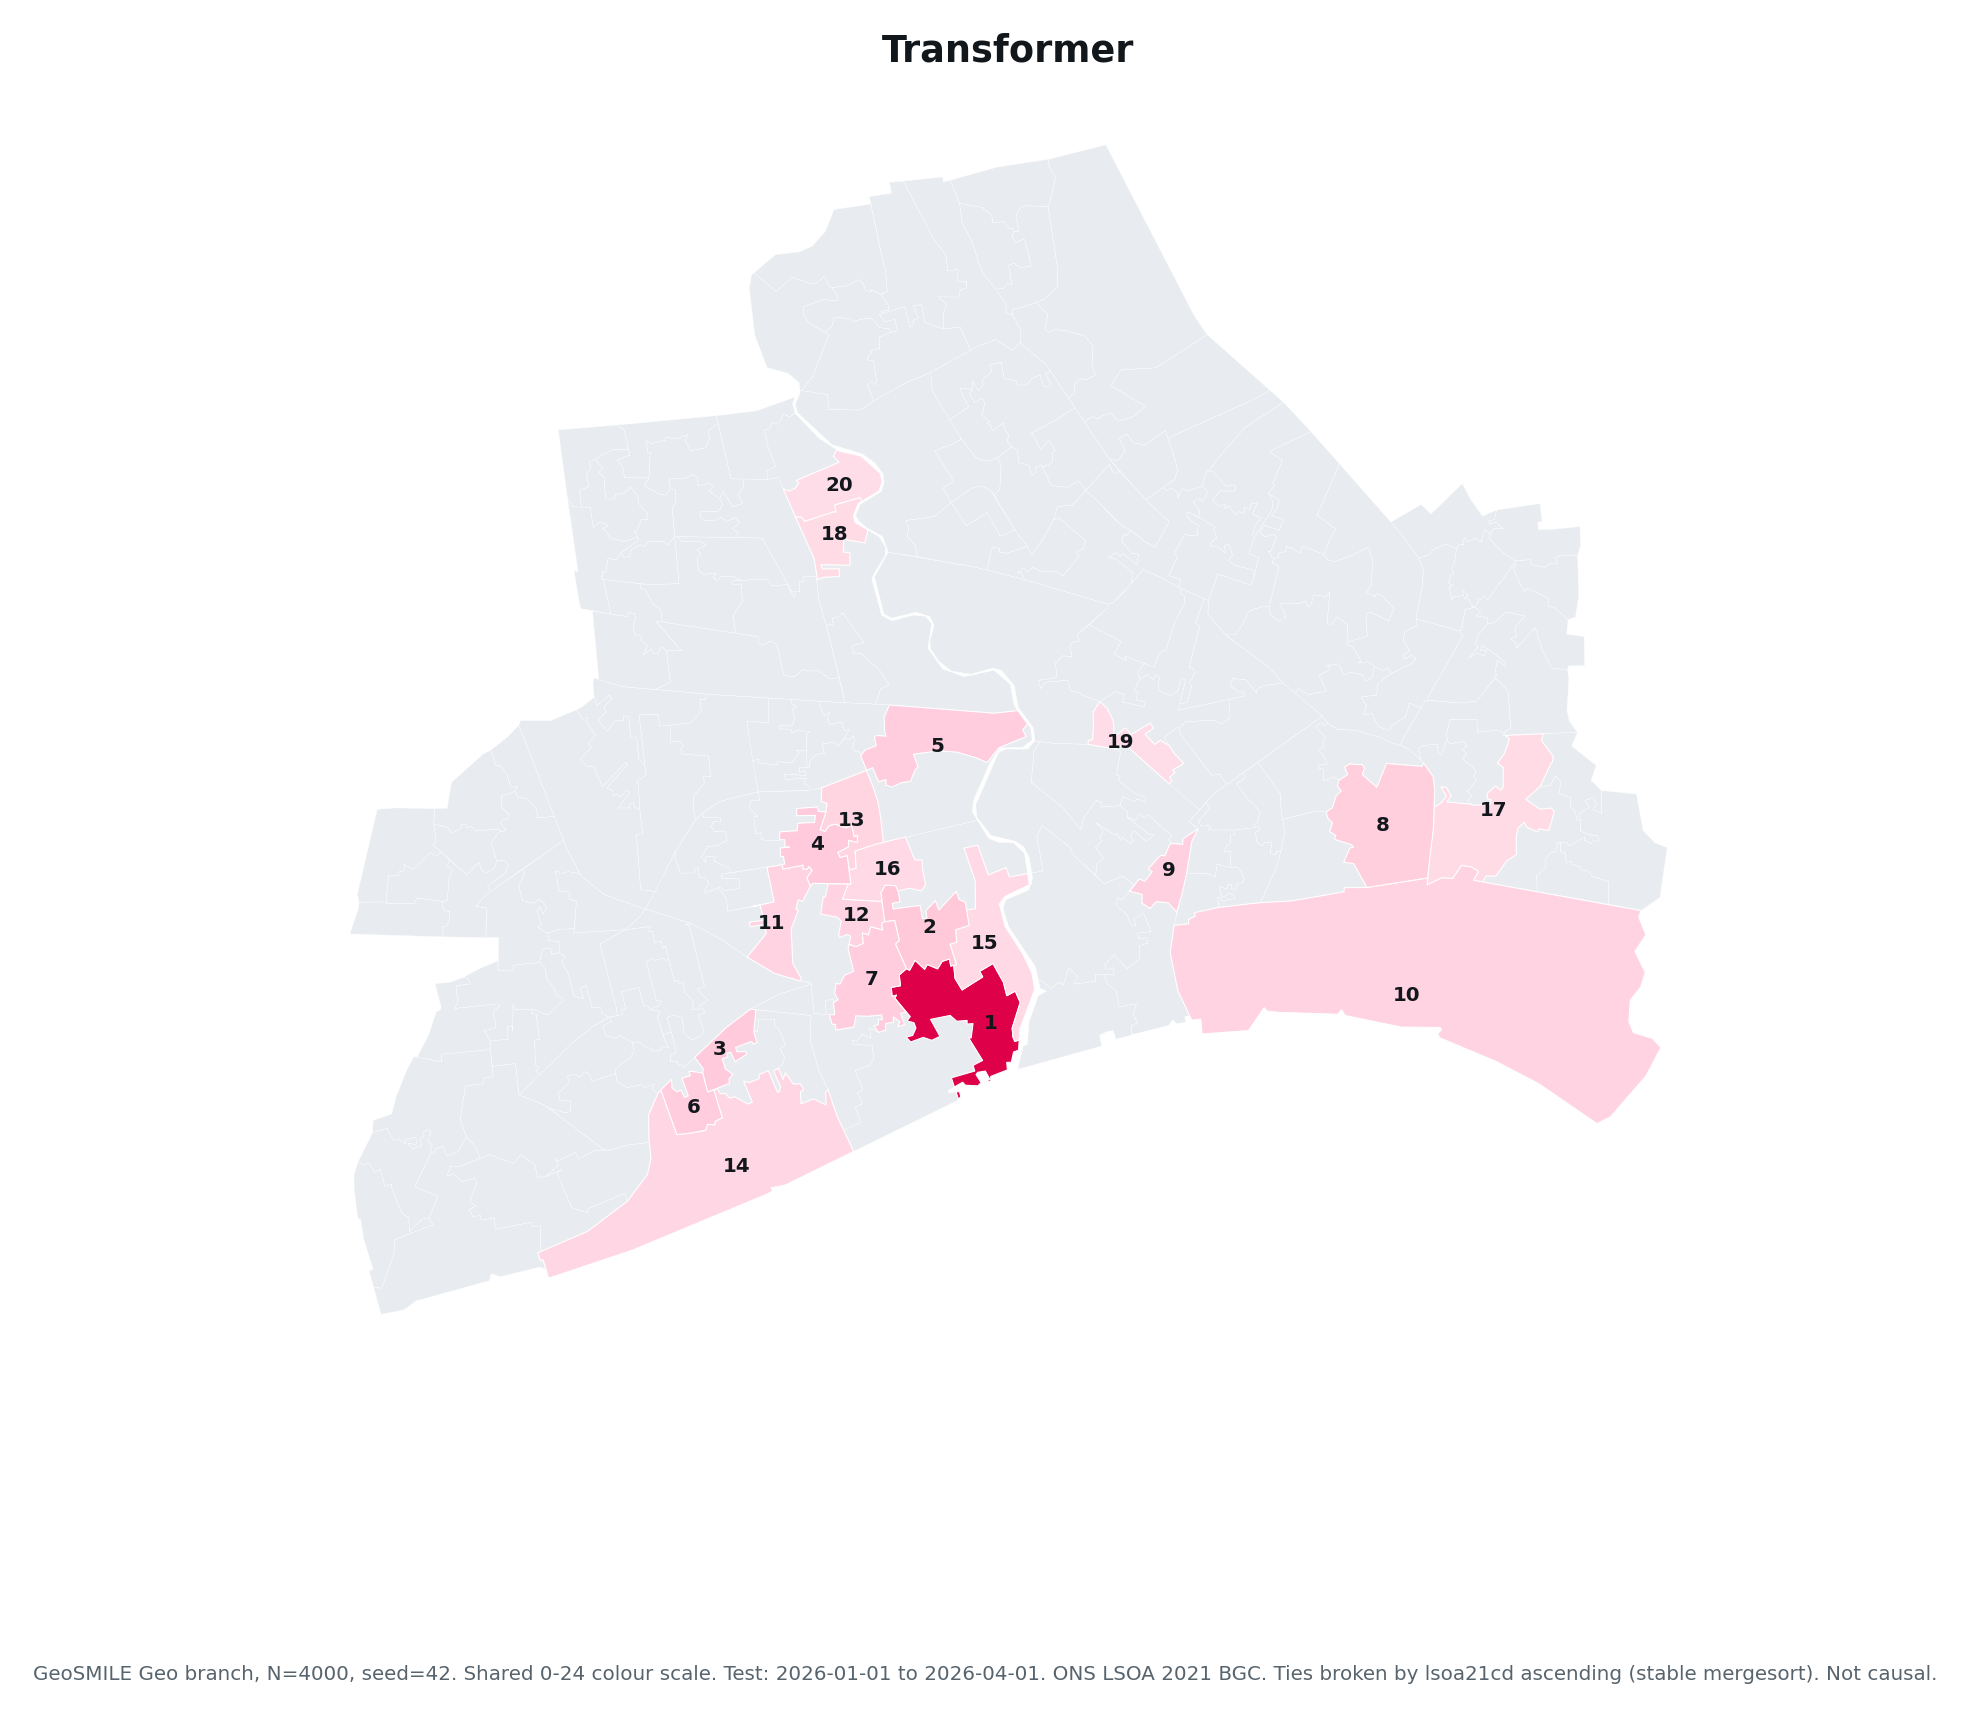
\includegraphics[width=\textwidth]{geo_top20_transformer_shared_scale.png}
    \subcaption{Transformer$^{\ddagger}$}
    \label{fig:sel_maps_transformer}
  \end{subfigure}

\vspace{0.8em}
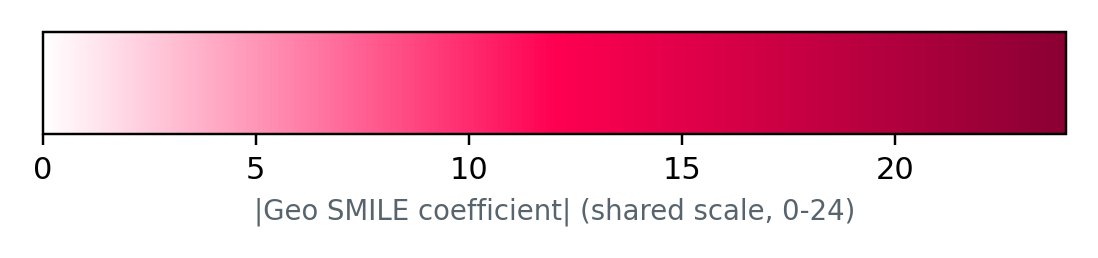
\includegraphics[width=0.55\textwidth]{shared_colorbar.png}

\caption{Geo SMILE top-20 LSOA attribution by candidate model, all eight
maps drawn on a shared |coefficient| colour scale (0--24) with one shared
colour bar so relative intensity is comparable across panels -- previously
each map was scaled to its own maximum (roughly 10 for ANN/CNN up to
roughly 23 for XGBoost/CatBoost), which would otherwise read as comparable
intensity when it was not. Rank labels 1--20 are unchanged. Geo $N{=}4{,}000$,
seed 42 for every panel; reconcile against Section~\ref{sec:hull_quant_results}
if that section reports $N{=}2{,}000$, as that describes an earlier design
point in this project. Superscripts mark provenance per
Table~\ref{tab:sel_provenance}: $\dagger$ saved from the rigorous
7-model verification (full metric suite); $\ddagger$ a fresh Ridge SMILE
fit for this round of design experiments (fidelity-focused only); $\S$ as
$\ddagger$, additionally forced through despite its own Geo-branch
predictive $R^2{=}0.661$ failing the $R^2>0.7$ guard.}
\label{fig:sel_maps}
\end{figure}
